%!TEX root = ../main.tex
\section{Decay time acceptance}
\label{sec:bd2jpsiks:decaytime:acceptance}

The trigger line requirements applied in the selection of the \BdToJPsiKS
candidates partially bias the decay time distribution. The sample is divided
into an \emph{almost unbiased} subset (AU), defined by
\begin{description}\small
  \item[AU] $\equiv$ \UseVerb{AlmostUnbiased}
\end{description}
and an \emph{exclusively biased} subset (EB), defined by
\begin{description}\small
  \item[EB] $\equiv$ \UseVerb{ExclusivelyBiased}
\end{description}
Here, the TOS decisions with respect to the \JPsi meson of these trigger lines
are used. For both samples the relative efficiency is calculated as the ratio
between the number of signal candidates fulfilling these trigger requirements
and those fulfilling the requirements of an unbiased collection of trigger
lines (\texttt{Hlt1DiMuonHighMass \&\& Hlt2DiMuonJPsi}). A simultaneous fit of
the mass distribution in ten bins of the decay time is performed to obtain the
signal yield ratios. The resulting histograms (see
\cref{fig:bd2jpsiks:decaytime:acceptance:splines}) are fitted with cubic
splines using the bin centres as knots for the splines. In the fit of the
spline function the bin contents are allowed to vary inside their
uncertainties, which are estimated as binomial errors for the AU sample and
via Gaussian error propagation for the EB sample. The acceptance shape at and
beyond the decay time limits is unknown, so it is assumed that the efficiency
shape is flat in front of the first and behind the last bin centre.

\begin{figure}[htb]
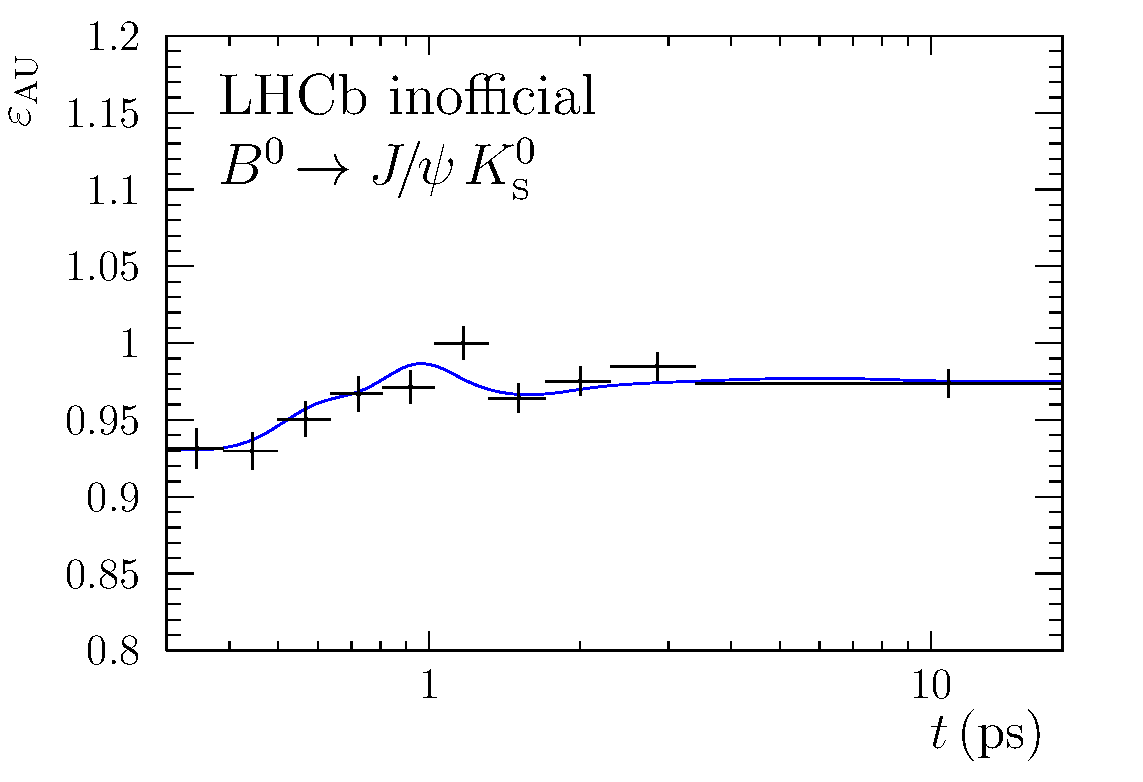
\includegraphics[width=0.49\textwidth]{06-Bd2JpsiKS/tikz/pdf/Acceptancespline_zoomed_hlt2.pdf}
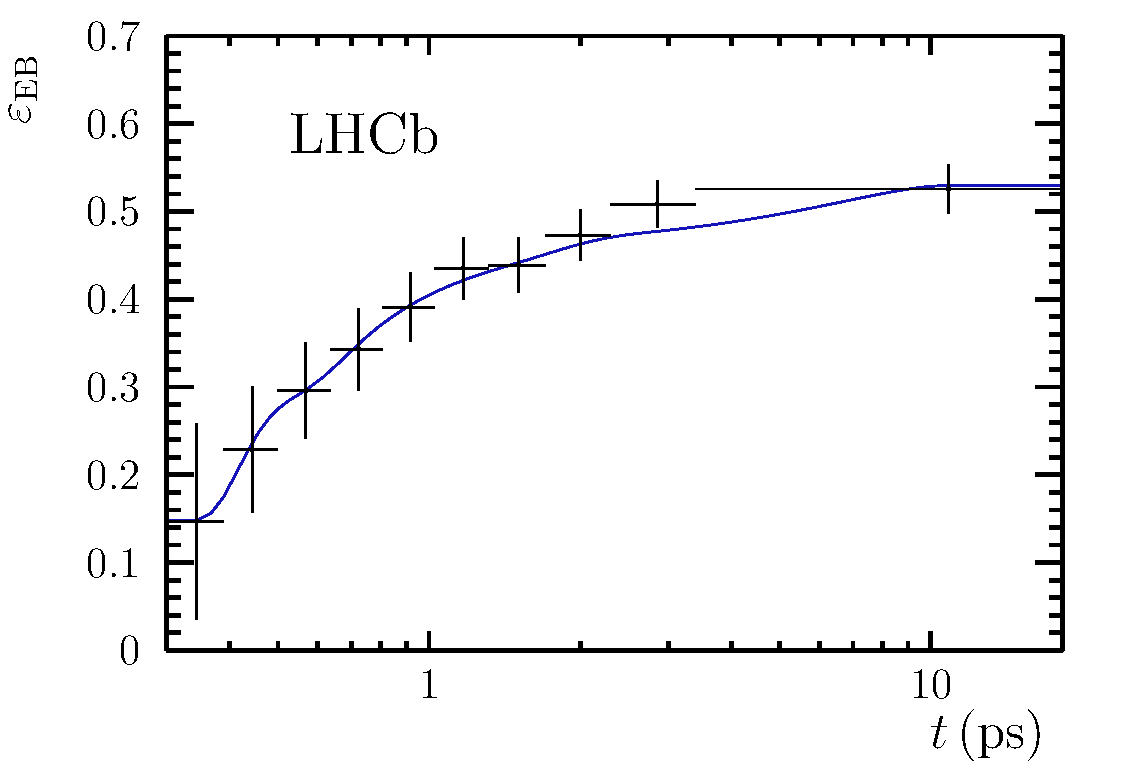
\includegraphics[width=0.49\textwidth]{06-Bd2JpsiKS/tikz/pdf/Acceptancespline_zoomed_hlt1.pdf}
\caption{Histograms of the trigger acceptance for the almost unbiased (left) and the
exclusively biased (right) sample. The blue curve shows the fitted acceptance
using splines.}
\label{fig:bd2jpsiks:decaytime:acceptance:splines}
\end{figure}

Another efficiency loss is observed at high decay times. This is mainly caused
by a reconstruction inefficiency of the VELO. To account for this effect the
lifetime $\tau$ is modified according to
\begin{equation}
  \widetilde{\tau} = \frac{\tau}{1 + \beta_\tau \tau}\,. 
\end{equation}
The correction factor $\beta_\tau$ is determined in a fit to simulated data,
where the generation value for the lifetime is known and thus can be fixed. To
avoid further decay-time biasing effects an unbiased sample is used. The
values, which are obtained individually for the two data-taking conditions and
the two track types, are listed in
\cref{tab:bd2jpsiks:decaytime:acceptance:beta}.
\begin{table}[htb]
	\centering
	\caption{Decay-time correction factor $\beta_\tau$ in \si{\invps}.}
	\begin{tabular}{ccc}
		\toprule
		 & 2011 & 2012 \\
		\midrule
		downstream & $0.0036\pm0.0029$ & $0.0084\pm0.0032$ \\
		long track & $0.018\pm0.004$   & $0.035\pm0.005$ \\
		\bottomrule
	\end{tabular}
	\label{tab:bd2jpsiks:decaytime:acceptance:beta}
\end{table}
It is apparent that the correction factors are roughly two times larger in
2012 than in 2011 and four to five times larger for long tracks than for
downstream tracks. While the former can be explained with changes in the
reconstruction software, the latter comparison clearly shows that the VELO is
the main reason for this acceptance effect.

\section{Decay time resolution}
\label{sec:bd2jpsiks:decaytime:resolution}

The most obvious effect of the decay time resolution are candidates that are
reconstructed with negative decay times. However, these are ideal candidates
to determine the decay time resolution. An unbinned likelihood fit to the
decay time distribution of an unbiased \BdToJPsiKS sample with true \JPsi
candidates (selected by a fit of the invariant $m_{\mumu}$ mass distribution)
is performed. The fit model consists of a component for the prompt peak around
\SI{0}{\ps}, \ie the decay time resolution model, a component to describe
events where a wrong PV has been associated and therefore a large difference
between true and reconstructed decay time occurs, and long-lived components.
The long-lived components are parametrised with two exponentials, which have
different pseudo lifetimes and which are themselves convolved with the decay
time resolution model. The decay time resolution depends on characteristics of
the event. The DTF provides predictions for the per-event decay time
resolution $\sigma_t$, which can be used as the width of a Gaussian resolution
model. However, these predictions are not perfect and a calibration needs to
be applied. Additionally, to account for different sources causing the decay
time resolution an effective model with two Gaussian functions, which share a
common mean but have different calibrations, is used.

The first step is to find a reasonable calibration model. A linear ($f_1$) and
a quadratic ($f_2$) calibration model are tested:
\begin{equation}
\begin{aligned}
f_1:&\quad \sigma_{\text{true}}(\sigma_t) &=&  &b_i\,\sigma_t &+ c_i \ , \\
f_2:&\quad \sigma_{\text{true}}(\sigma_t) &=&\, \alpha_i\,\sigma_t^2 + &\beta_i\,\sigma_t &+ \gamma_i \ .
\end{aligned}
\label{eq:resolutioncalibfunctions}
\end{equation}
%
The data sample is divided into \num{20} equally filled bins of the decay time
resolution predictions $\sigma_t$. This is done separately for the downstream
and the long track sample as the decay time resolution of long track
candidates is expected to be significantly better. Under the assumption that
$\sigma_t$ is constant inside the bins average widths can be set for the two
Gaussian functions. An unbinned likelihood fit to the decay time distribution,
simultaneous in all bins, sharing all fit parameters except the widths of the
Gaussian resolution functions is performed. The widths are plotted in the
corresponding bins and a \chisq-fit with the two calibration functions is
executed. For the downstream sample the results are depicted in
\cref{fig:CalibrationOffsetResolution_DD}.
%
\begin{figure}[!htb]
\centering
  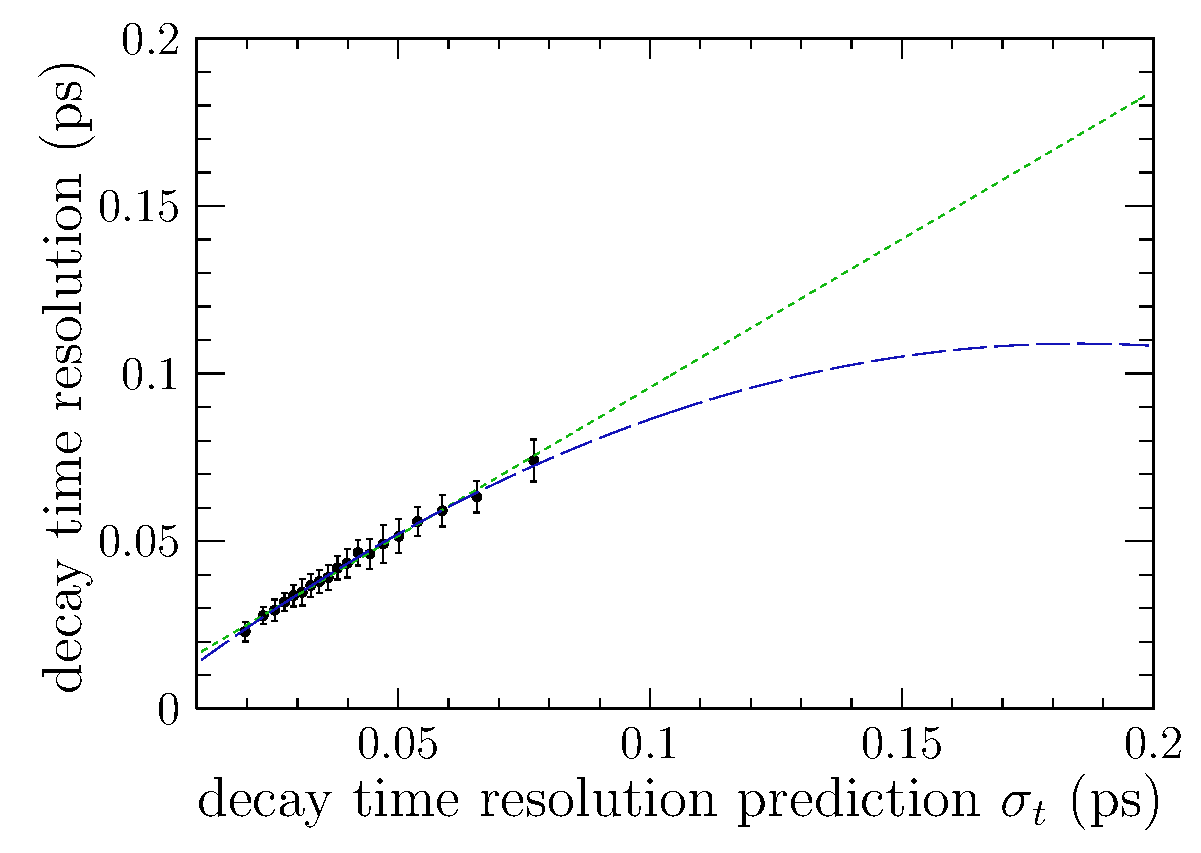
\includegraphics[width=0.45\textwidth]{06-Bd2JpsiKS/tikz/pdf/ResolutionCalibration_1_DD.pdf}
  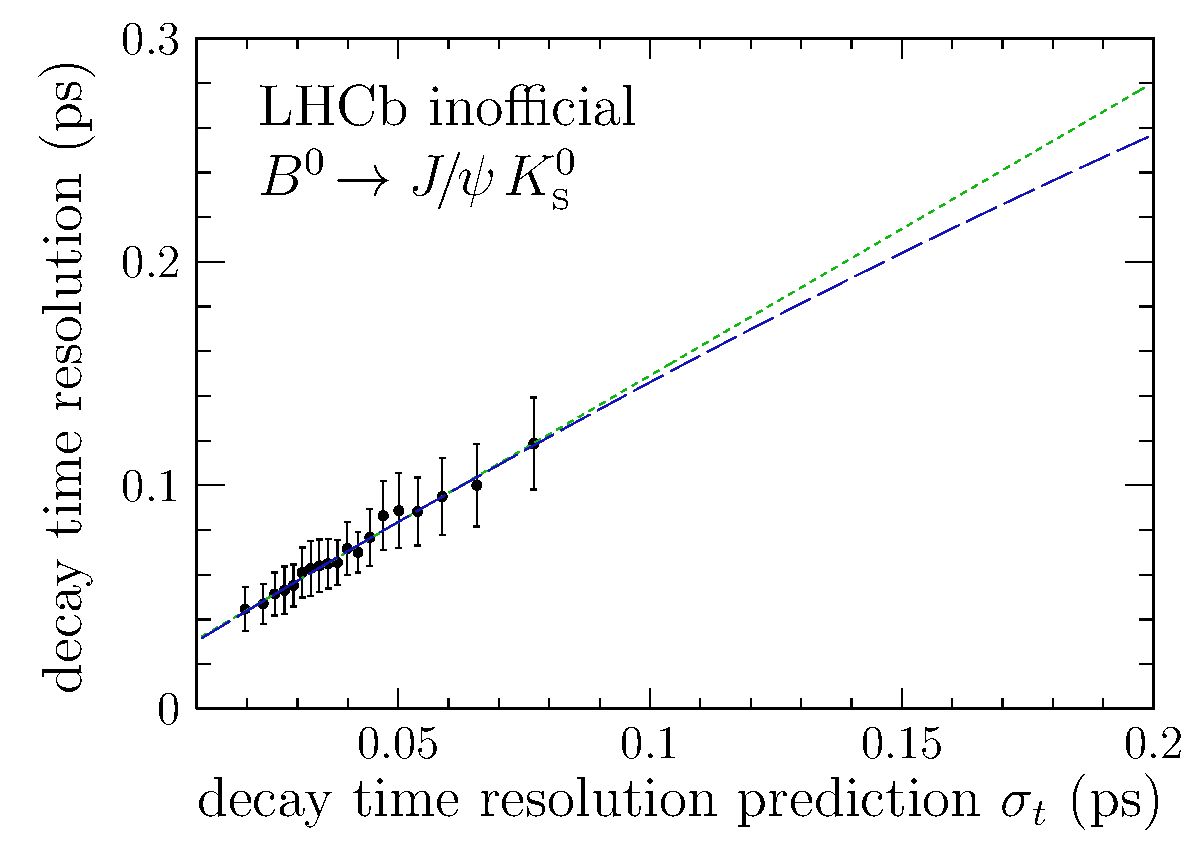
\includegraphics[width=0.45\textwidth]{06-Bd2JpsiKS/tikz/pdf/ResolutionCalibration_2_DD.pdf}
\caption{Fit of a linear (green short-dashed) and a quadratic calibration
function (blue long-dashed) to the narrower (left) and to the wider width
(right) of the downstream sample.}
\label{fig:CalibrationOffsetResolution_DD}
\end{figure}
%
Both functions fit equally well, so the simpler linear model with less degrees
of freedom is preferred. The linear model is also chosen for the long track
sample.

With the calibration functions at hand an unbinned likelihood fit in decay
times and decay time resolution predictions is performed and the nominal
values of the calibration parameters are determined. The dilution factor
induced by the decay time resolution (see
\cref{eq:dataanalysis:resolution:dilution}) is calculated to be \num{0.986}
for downstream and \num{0.989} for long track candidates.